\documentclass[12pt]{article}

\usepackage{sbc-template}
\usepackage{graphicx,url}
\usepackage[utf8]{inputenc}
\usepackage{multicol}
\usepackage{listings}
\usepackage{xcolor}

\definecolor{codegreen}{rgb}{0,0.6,0}
\definecolor{codegray}{rgb}{0.5,0.5,0.5}
\definecolor{codepurple}{rgb}{0.58,0,0.82}
\definecolor{backcolour}{rgb}{0.95,0.95,0.92}

\lstdefinestyle{mystyle}{
    backgroundcolor=\color{backcolour},   
    commentstyle=\color{codegreen},
    keywordstyle=\color{magenta},
    numberstyle=\tiny\color{codegray},
    stringstyle=\color{codepurple},
    basicstyle=\ttfamily\footnotesize,
    breakatwhitespace=false,         
    breaklines=true,                 
    captionpos=b,                    
    keepspaces=true,                 
    numbers=left,                    
    numbersep=5pt,                  
    showspaces=false,                
    showstringspaces=false,
    showtabs=false,                  
    tabsize=2
}

\lstset{style=mystyle}
   
\sloppy

\title{AED II - Unidade 03 - Fundamentos de }

\author{Luca Ribeiro Schettino Regne}

\begin{document} 

\maketitle

\section{Exercícios Resolvidos}
\subsection{Resolva as equações abaixo:}
a)$ 2^{10} = 1024$\\
b)$ lg(1024) = 10$\\
c)$ lg(17) = 	4,0875 $\\
d)$ \lceil{lg(17)}\rceil = 5$\\
e)$ \lfloor{lg(17)}\rfloor  = 4$

\subsection{Plote um gráfico com todas as funções abaixo)
a)$f(n) = n^{3} $\\
b)$f(n) = n^{2}$\\
c)$f(n) = n x lg(n)$\\
d)$f(n) = n$\\
e)$f(n) = sqrt(n)$\\
f)$f(n) = lg(n)$\\\\
\begin{figure}[h]
    \centering
    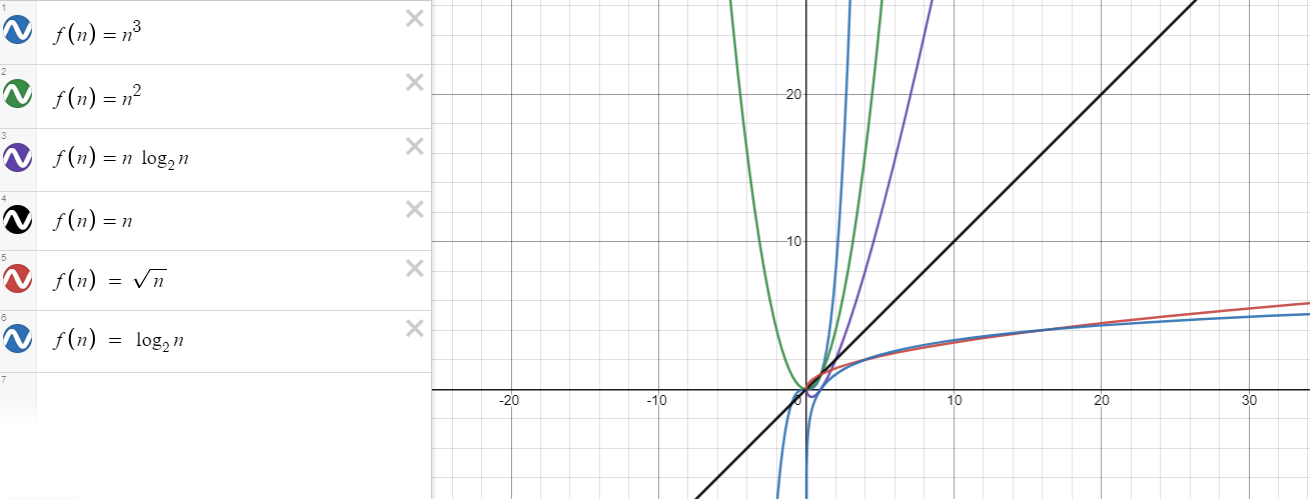
\includegraphics[width=1\textwidth]{images/graph.png}
\end{figure}

\subsection{Calcule o número de subtrações que o código abaixo realiza:}
\begin{lstlisting}[language=Java]
    ...
    for (int i = 0; i < n; i++){
        if (i % 2 == 0){
            a--;
            b--;
        } else{
            c--;
        }
    }
\end{lstlisting}
Melhor caso: $f(n) = 2n (O(n), \Theta(n), \Omega(n))$
Pior caso: $f(n) = 2n (O(n), \Theta(n), \Omega(n))$

\subsection{Calcule o número de subtrações que o código abaixo realiza:}
\begin{lstlisting}[language=Java]
    ...
    for (int i = 3; i < n; i++){
        if (i % 2 == 0){
            a--;
        }
    }
\end{lstlisting}
Subtrações = $n - 3$ .\\ $O(n)$, $\Theta(n)$, $\Omega(n)$

\subsection{Calcule o número de multiplicações que o código abaixo realiza:}
\begin{lstlisting}
    for(int i = n; i > 2; i /= 2){
        a *= 2;
    }
\end{lstlisting}
Multiplicações = $\lceil lg(n) \rceil + 1$\\ $O(lg n)$, $\Theta(lg n)$ e $\Omega(lg n)$

\subsection{Outra forma de compreender o código anterior é executando o mesmo}
\begin{lstlisting}[language=Java]
    class Log {
        public static void main (String[] args){
            int[] n = {4,5,6,7,8,9,10,11,12,13,14,15,16,17,31,32,33,63,64,65};
            int cont;
            for(int k = 0; k < n.length; k++){
                System.out.print("\n[n = " + n[k] + "] => ");
                cont = 0;
                for(int i = n[k]; i > 0; i /= 2){            
                    System.out.print(" " + i);
                    cont++;
                }
                System.out.print(" (" + cont + " vezes)");
            }
            System.out.print("\n");
        }
    }
\end{lstlisting}

\subsection{Encontre o menor valor em um array de inteiros}
\begin{lstlisting}[language=Java]
    int min = array[0];
    for (int i = 1; i < n; i++){
        if (min > array[i]){
            min = array[i];
        }
    }
\end{lstlisting}
1. Qual é a operação relevante?\\
Comparação entre elementos do array\\\\
2.Quantas vezes ela será executada?\\
Se tivermos n elementos: T(n) = n - 1\\\\
3.O nosso T(n) = n – 1 é para qual dos três casos?\\
Para todos os casos. $O(n)$, $\Theta(n)$, $\Omega(n)$\\

\subsection{Encontrar Mínimo}
\begin{lstlisting}
    int min = array[0];
    for (int i = 1; i < n; i++){
        if (min > array[i]){
            min = array[i];
        }
    }
\end{lstlisting}
1º) Qual é a operação relevante?\\
Comparação entre elementos do array\\\\
2º) Quantas vezes ela será executada?\\
Se tivermos n elementos: T(n) = n - 1\\\\
3º) O nosso T(n) = n – 1 é para qual dos três casos?\\
Para os três casos\\\\
4º) O nosso algoritmo é ótimo? Por que?\\
Sim, porque temos que testar todos os elementos para garantir nossa resposta

\subsection{Pesquisa Sequencial}
\begin{lstlisting}
    boolean resp = false;
    for (int i = 0; i < n; i++){
        if (array[i] == x){
            resp = true;
            i = n;
        }
    }
\end{lstlisting}
1º) Qual é a operação relevante?\\
Comparação entre elementos do array\\\\
2º) Quantas vezes ela será executada?\\
Melhor caso: f(n) = 1
   \\Pior caso: f(n) = n
   \\Caso médio: f(n) = (n + 1) / 2\\\\
3º) O nosso algoritmo é ótimo? Por que?\\
Sim porque temos que testar todos os elementos para garantir nossa resposta.

\subsection{Um aluno deve procurar um valor em um array de números reais. Ele tem duas alternativas. Primeiro, executar uma pesquisa sequencial. Segundo, ordenar o array e, em seguida, aplicar uma pesquisa binária. O que fazer?}
O aluno deve escolher a primeira opção, pois a pesquisa sequencial tem custo $\Omega(n)$. A segunda opção tem custo $\Omega(n * lg n)$ para ordenar mais $\Omega(lg n)$ para a pesquisa binária.

\subsection{Responda se as afirmações são verdadeiras ou falsas:}
a)$3n^2 + 5n + 1$ é $O(n)$: Falsa\\\\
b)$3n^2 + 5n + 1$ é $O(n^2)$: Verdadeira\\\\
c)$3n^2 + 5n + 1$ é $O(n^3)$: Falsa\\\\
d)$3n^2 + 5n + 1$ é $\Theta(n)$: Falsa\\\\
e)$3n^2 + 5n + 1$ é $\Theta(n^2)$: Verdadeira\\\\
f)$3n^2 + 5n + 1$ é $\Theta(n^3)$: Verdadeira\\\\
g)$3n^2 + 5n + 1$ é $\Omega(n)$: Falsa\\\\
h)$3n^2 + 5n + 1$ é $\Omega(n^2)$: Verdadeira\\\\
i)$3n^2 + 5n + 1$ é $\Omega(n^3)$: Falsa\\\\

\subsection{Apresente a função e a complexidade para os números de comparações e movimentações de registros para o pior e melhor caso}
\begin{lstlisting}
    void imprimirMaxMin(int[] array, int n){
        int maximo, minimo;
        if (array[0] > array[1]){
            maximo = array[0];
            minimo = array[1];
        }else{
            maximo = array[1];
            minimo = array[0];
        }
        
        for(int i = 2; i < n; i++){
            if (array[i] > maximo){
                maximo = array[i];
            } else if(array[i] < minimo){
                minimo = array[i];
            }
        }
    }
\end{lstlisting}
\begin{center}
    Função de complexidade - MOV
\end{center}
PIOR: $f(n) = 2 + (n – 2)$\\
MELHOR: $f(n) = 2 + (n – 2) x 0$\\
\begin{center}
    Complexidade - MOV
\end{center}
PIOR: $O(n)$, $\Theta(n)$ e $\Omega(n)$\\
MELHOR: $O(1)$, $\Theta(1)$ e $\Omega(1)$\\
\begin{center}
    Função de complexidade - CMP
\end{center}
PIOR: $f(n) = 1 + 2(n – 2)$\\
MELHOR: $f(n) = 1 + (n – 2)$\\
\begin{center}
    Complexidade - CMP
\end{center}
PIOR: $O(n)$, $\Theta(n)$ e $\Omega(n)$\\
MELHOR: $O(n)$, $\Theta(n)$ e $\Omega(n)$\\

\subsection{Apresente a função e a complexidade para o número de subtrações para o pior e melhor caso}
\begin{lstlisting}
    i = 0;
    while (i < n) {
        i++;
        a--;
    }
    
    if (b > c) {
        i--;
    } else {
        i--;
        a--;
    }
\end{lstlisting}

\begin{center}
    Função de complexidade
\end{center}
PIOR: $f(n) = n + 2$ \\
MELHOR: $f(n) = n +1$
\begin{center}
    Complexidade
\end{center}
PIOR: $O(n)$, $\Theta(n)$ e $\Omega(n)$\\
MELHOR: $O(n)$, $\Theta(n)$ e $\Omega(n)$

\subsection{Apresente a função e a complexidade para o número de subtrações para o pior e melhor caso}
\begin{lstlisting}
    for (i = 0; i < n; i++) {
        for (j = 0; j < n; j++) {
            a--;
            b--;
        }
        c--;
    }
\end{lstlisting}
Função de complexidade: $f(n) = (2n + 1)n$\\
Complexidade: $O(n^2)$, $\Theta(n^2)$ e $\Omega(n^2)$

\subsection{Apresente a função e a complexidade para o número de subtrações para o pior e melhor caso} 
\begin{lstlisting}
    for (i = 0; i < n; i++) {
        for (j = 1; j <= n; j *= 2) {
            b--;
        }
    }
\end{lstlisting}
Função de complexidade: $f(n) = (lg(n) + 1) * n = n * lg(n) + n$
Complexidade: $O(n x lg(n))$, $\Theta(n x lg(n))$ e $\Omega(n x lg(n))$

\subsection{Apresente a função e a complexidade para o número de subtrações para o pior e melhor caso}
\begin{lstlisting}
    for (i = 0; i < n; i++) {
        for (j = 1; j <= n; j *= 2) {
            b--;
        }
    }
\end{lstlisting}
Função de complexidade: $(lg(n) + 1) * n = n * lg(n) + n$\\
Complexidade: $O(n x lg(n))$, $\Theta(n x lg(n))$ e $\Theta(n x lg(n))$

\subsection{Apresente o tipo de crescimento que melhor caracteriza as funções abaixo}
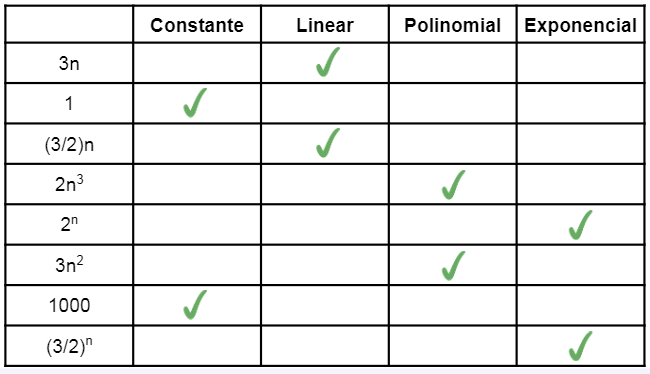
\includegraphics{images/exercicio_16.png}

\subsection{Classifique as funções f1(n) = n2, f2(n) = n, f3(n) = 2n, f4(n) = (3/2)n, f5(n) = n3e f6(n) = 1 de acordo com o crescimento, do mais lento para o mais rápido}
$f_{6}(n) = 1$
\\$f_{2}(n) = n$
\\$f_{1}(n) = n^2$
\\$f_{5}(n) = n^3$
\\$f_{4}(n) = (3/2)^n$
\\$f_{3}(n) = 2n$

\subsection{Classifique as funções f1(n) = n.log6(n), f2(n) = lg(n), f3(n) = log8(n), f4(n) = 8n2, f5(n) = n.lg(n), f6(n) = 64, f7(n) = 6n3, f8(n) = 82n e f9(n) = 4n de acordo com o crescimento, do mais lento para o mais rápido}
$f_{6}(n) = 64$
\\$f_{3}(n) = log_{8}(n)$
\\$f_{2}(n) = lg(n)$
\\$f_{9}(n) = 4n$
\\$f_{1}(n) = n.log6(n)$
\\$f_{5}(n) = n.lg(n)$
\\$f_{4}(n) = 8n^2$
\\$f_{7}(n) = 6n^3$
\\$f_{8}(n) = 8^{2n}$

\subsection{Faça a correspondência entre cada função f(n) com sua g(n) equivalente, em termos de 𝚯. Essa correspondência acontece quando f(n) = 𝚯(g(n))}
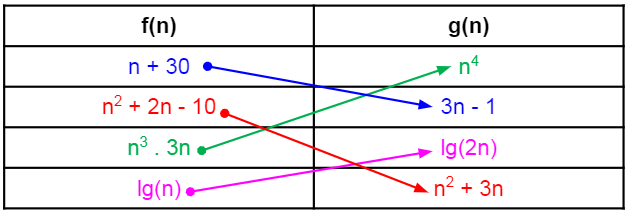
\includegraphics{images/exercicio_19.png}

\section{Exercícios}
\subsection{Encontre o maior e menor valores em um array de inteiros e, em seguida, encontre a função de complexidade de tempo para sua solução}

\subsection{Considerando o problema de encontrar o maior e menor valores em um array de inteiros, veja os quatro códigos propostos e analisados no livro do Ziviani}

\subsection{Preencha verdadeiro ou falso na tabela abaixo:}
\begin{table}[htb]
    \begin{tabular}{|l|l|l|l|l|l|l|l|} \hline
                              & $O(lg n)$ & $O(n)$ & $O(n.lg(n))$ & $O(n^2)$ & $O(n^3)$ & $O(n^5)$ & $O(n^20)$ \\ \hline
    $f(n) = lg(n)$            &          &         &              &          &          &          &           \\ \hline
    $f(n) = n . lg(n)$        &          &         &              &          &          &          &           \\ \hline
    $f(n) = 5n + 1$           &          &         &              &          &          &          &           \\ \hline
    $f(n) = 7n^5 - 3n^2$      &          &         &              &          &          &          &           \\ \hline
    $f(n) = 99n^3 - 1000n^2$  &          &         &              &          &          &          &           \\ \hline
    $f(n) = n^5 - 99999n^4$   &          &         &              &          &          &          &           \\ \hline
    \end{tabular}
\end{table}

\subsection{Preencha verdadeiro ou falso na tabela abaixo:}
\begin{table}[htb]
    \begin{tabular}{|l|l|l|l|l|l|l|l|} \hline
                              & $\Theta(lg n)$ & $\Theta(n)$ & $\Theta(n.lg(n))$ & $\Theta(n^2)$ & $\Theta(n^3)$ & $\Theta(n^5)$ & $\Theta(n^20)$ \\ \hline
    $f(n) = lg(n)$            &                &             &                   &               &               &               &                \\ \hline
    $f(n) = n . lg(n)$        &                &             &                   &               &               &               &                \\ \hline
    $f(n) = 5n + 1$           &                &             &                   &               &               &               &                \\ \hline
    $f(n) = 7n^5 - 3n^2$      &                &             &                   &               &               &               &                \\ \hline
    $f(n) = 99n^3 - 1000n^2$  &                &             &                   &               &               &               &                \\ \hline
    $f(n) = n^5 - 99999n^4$   &                &             &                   &               &               &               &                \\ \hline
    \end{tabular}
\end{table}

\subsection{Preencha verdadeiro ou falso na tabela abaixo:}
\begin{table}[htb]
    \begin{tabular}{|l|l|l|l|l|l|l|l|} \hline
                              & $\Omega(lg n)$ & $\Omega(n)$ & $\Omega(n.lg(n))$ & $\Omega(n^2)$ & $\Omega(n^3)$ & $\Omega(n^5)$ & $\Omega(n^20)$ \\ \hline
    $f(n) = lg(n)$            &                &             &                   &               &               &               &                \\ \hline
    $f(n) = n . lg(n)$        &                &             &                   &               &               &               &                \\ \hline
    $f(n) = 5n + 1$           &                &             &                   &               &               &               &                \\ \hline
    $f(n) = 7n^5 - 3n^2$      &                &             &                   &               &               &               &                \\ \hline
    $f(n) = 99n^3 - 1000n^2$  &                &             &                   &               &               &               &                \\ \hline
    $f(n) = n^5 - 99999n^4$   &                &             &                   &               &               &               &                \\ \hline
    \end{tabular}
\end{table}

\subsection{Dado $f(n)=3n^2-5n-9$,$g(n)=n*lg(n)$,$l(n)=n.lg^2(n)$ e $h(n)=99n^8$, qual é a ordem de complexidade das operações:}
a)f(n) + g(n) - h(n)\\
b)O(f(n) + O(g(n)) - O(h(n))\\
c)f(n) x g(n)\\
d)g(n) x l(n) + h(n)\\
e)f(n) x g(n) x l(n)\\
f)O(O(O(O(f(n)))))\\
\end{document}
